\section{\color{blue}Guaranteeing Consensus of Double Integrators in Presence of a Directed Cycle}\label{Conc:Approach1}
\begin{frame}
	\begin{block}{Results from approach 1}
		\begin{enumerate}
			\item We were able to achieve better sufficiency condition than the one in the literature.\hyperlink{BetterSuff}{\beamerbutton{Theorem}}
			\item We proposed a polynomial-based approach where the roots are determined by the cycle in the loop, and the real root alone is sufficient to compute the sufficiency condition.
			\item The lengths of cycle and their relative positions are sufficient for finding the bound and is independent of the network size. 
		\end{enumerate}
	\end{block}
	\begin{block}{Challenges in Approach 1:}
		\begin{enumerate}
			\item The polynomial-based approach fails to analyze scenarios where the leader is part of the directed cycle.
			\item It simplifies computation but does not help in reducing or eliminating the bound.
			\item Not a local remedy as requires every agent to update the $\gamma$ value to achieve consensus.
		\end{enumerate}
	\end{block}
	\textcolor{blue}{Publications: }\\
	\begin{enumerate}
		\item Dubey, A. K., Mukherjee, D., \& Arya, K. (2022). Consensus of double integrators over a chain with reverse edges. IFAC-PapersOnLine, 55(13), 19-24.
	\end{enumerate}
	%\pause
	%\centering So can't we reduce the bound? \pause~~~\textcolor{blue}{Yes, We can}\\
	\vspace{0.2cm}
\end{frame}

\begin{frame}{Approach 2: Edge Weight Perturbation}\label{gersback}
	%\textcolor{blue}{Methodology} Using edge weight perturbation of the cycles and/or neighboring edge to the cycle, to 
	\textcolor{brown}{Guaranteed the consensus} for any pre-designed velocity coupling factor.\\ %Not only \textcolor{cyan}{for the leaderless case} but also for the case where \textcolor{cyan}{the directed cycle involves leader}.
	%\begin{itemize}
		%\item 
		-- \textcolor{blue}{Directed cycle without leader} $\rightarrow$ Guaranteed the consensus using the Node Scaling, the Edge Scaling and the combined scaling methods utilizing the Gershgorin's disc theorem. 
				\begin{columns}
					\begin{column}{0.5\textwidth}
						\begin{figure}
							\centering
							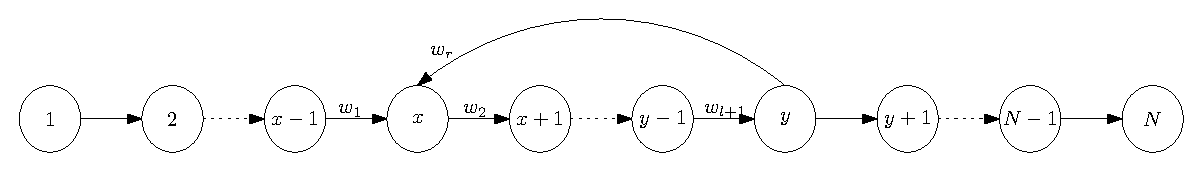
\includegraphics[scale=0.35,keepaspectratio]{Images/EdgeScaling.eps}
							\caption{Edge Scaling Method}
							%\label{EdgeScaledNetwork}
						\end{figure}
					\end{column}
					\begin{column}{0.5\textwidth}
						\begin{figure}
							\centering
							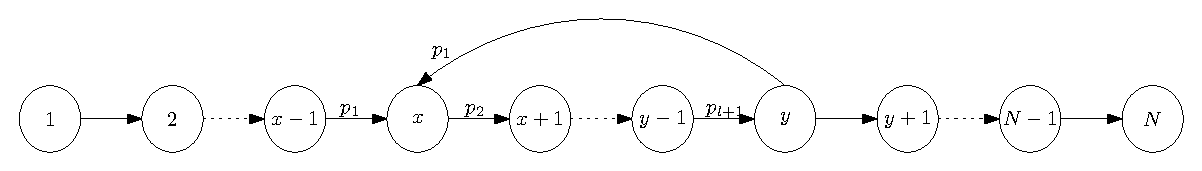
\includegraphics[scale=0.35,keepaspectratio]{Images/NodeScaling.eps}
							\caption{Node Scaling method}
							%\label{EdgeScaledNetwork}
						\end{figure}
					\end{column}
				\end{columns}
		%\item For directed cycle with leader $\rightarrow$ Root Locus Based approach.
	%\end{itemize}
	\hyperlink{NSSimbase}{\beamerbutton{{NS Method}}}~~\hyperlink{ESSimbase}{\beamerbutton{{ES Method}}}~~\hyperlink{CombScal}{\beamerbutton{{NES Method}}}~~ \hyperlink{gers}{\beamerbutton{Gershgorin's Theorem}}\\
	\pause
	-- \textcolor{blue}{Directed cycle with leader}
	\begin{itemize}
		\item Guranteed the consensus for a situation that has not been analyzed enough in the literature.
		\item Utilized a simple root locus based strategy, again applicable locally, to mitigate the adverse effects of the reverse edge.\hyperlink{RLSimbase}{\beamerbutton{RLS Method}}
		\item Contrary to the node scaling and the edge scaling methods, where increasing the scaling parameters assists in consensus, here one of the gain $\beta$ needs to be bounded above, while the other gain $\alpha$ is to be chosen large for achieving the consensus.
	\end{itemize}
	%\begin{block}{Future Work}
	%	\begin{itemize}
	%		\item To obtain a tighter lower bound on the coupling factor $\gamma$ by using both the real and imaginary parts of the eigenvalues.
	%		\item Considering more general types of directed acyclic graphs also remains an important problem to be addressed within this set-up.
	%	\end{itemize}
	%\end{block}
\end{frame}
%%%%%%%%%%%%%%%%%%%%%%%%%%%%%%%%%%%%%%%%%%%%%%%%%%%%%%%%%%%%%%%%%%%%%%%%%%%%%%%%%%
\begin{frame}
	\begin{block}{Conclusion}
		\begin{itemize}
			\item Guaranteed consensus for any pre-designed value of $\gamma$ .
			\item Can be applied locally and the agents outside the directed cycle need not alter their control laws.
			\item Adressed the case when the leader in the chain is forced into a directed cycle, a situation that has not been analyzed enough in the literature.
		\end{itemize}
	\end{block}
	\textcolor{blue}{Publications: }\\
	\begin{enumerate}
		\item Dubey, A. K., Mukherjee, D., \& Arya, K. (2023, May). Consensus of double integrators in presence of a reverse edge in a chain: Analysis and design. In 2023 American Control Conference (ACC) (pp. 411-416). IEEE.
		\item Dubey, A. K. \& Mukherjee, D.(2024). Guaranteed Consensus in System of Double Integrators in Presence of Directed Cycles [Journal to be communicated]
	\end{enumerate}
\end{frame}

\begin{subframe}{}
	Why Gershgorin's Theorem work??\\ 
	\pause
	The $\gamma$ bound is characterized by the eigenvalues of matrix $\mathcal{C}$ as:
	$$\mathcal{L}=\begin{bmatrix}
		\mathcal{L}_1 & 0 & 0 \\
		* & \mathcal{C} & 0 \\
		* & * & \mathcal{L}_2
	\end{bmatrix}\text{ (without Leader)}$$
	\vspace{-0.1cm}
	\begin{block}{New Sufficiency Condition}
		$$\gamma \geq \frac{1}{\sqrt{\lambda_1}}$$
		- $\lambda_1$ is the one and only real eigenvalue\\ 
		- $\lambda_1$ is the lowest real eigenvalue
	\end{block}
	\vspace{-0.1cm}
	\begin{exampleblock}{}
		- Zero eigenvalue is part of $\mathcal{L}_1$\\
		- Eigenvalue of $\mathcal{C}$ is all positive.
	\end{exampleblock}
	\vspace{-0.1cm}
	\begin{alertblock}{}
		- Row Picture of Gershgorin's Discs always touches zero\\
		- However, Column Picture of Gershgorin's Discs may not
	\end{alertblock}
	%\textbf{Note 1:} Although the Gershgorin's Discs always touches zero when looking at the row picture but we can ensure that the Gershgorin's discs do not touch zero while looking at the column picture. 
	\hyperlink{Conc:Approach1}{\beamerbutton{Approach1}}
\end{subframe}


\begin{subframe}{Node Scaled Method}\label{NSSimbase}	
	\begin{figure}
		\centering
		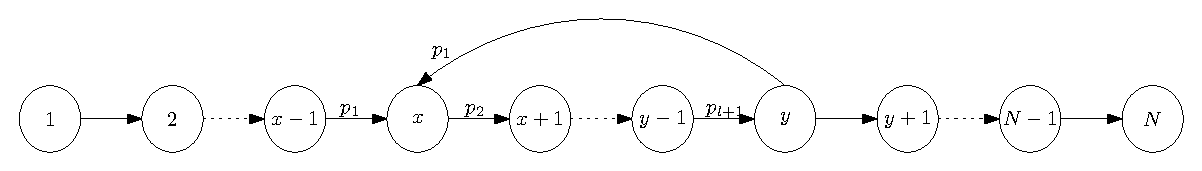
\includegraphics[scale=0.35,keepaspectratio]{Images/NodeScaling.eps}\\
		%\caption{Node Scaled Network}
		%\label{NodeScaledNetwork}
	\end{figure}
	%\pause
	$\Tilde{P}=P\mathcal{C}=\tiny{\begin{bsmallmatrix}
		2p_1  & 0  & \dots & -p_1 \\
		-p_2 & p_2 & \dots & 0 \\
		\vdots & \vdots & \ddots & \vdots \\
		\vdots & \dots & -p_{(\ell+1)} & p_{(\ell+1)}
	\end{bsmallmatrix}},$
	where, $P=\text{diag}(p_1,p_2,p_3,\dots,p_{\ell+1})$ is a matrix with positive entries.
	\vspace{-0.2cm}
	\begin{block}{Objective}
		Applying Gershgorin's Disc theorem to columns 
		$$2p_1>p_2>p_3>\dots>p_{\ell+1}>p_1$$
		
		- Ensure it is separated from origin \\
		- Maximize the distance of closest disc\\
		\textcolor{blue}{Solution: }Create an Arithmetic Progression between the elements of inequality above.
	\end{block}
	Consensus is achieved if:		$p_{i-x_1+1}=\frac{\ell+1}{\gamma^2}+\epsilon+(i-x_1)\frac{[(\ell+1)/\gamma^2]+\epsilon}{\ell+1}, \epsilon>0.$ \hyperlink{NSSim}{\beamerbutton{Simulations}}~~\hyperlink{gersback}{\beamerbutton{Back2Approach2}}
\end{subframe}



\begin{subframe}{Edge Scaled Method}\label{ESSimbase}
	%\begin{minipage}{0.45\textwidth}
	\begin{figure}
		\centering
		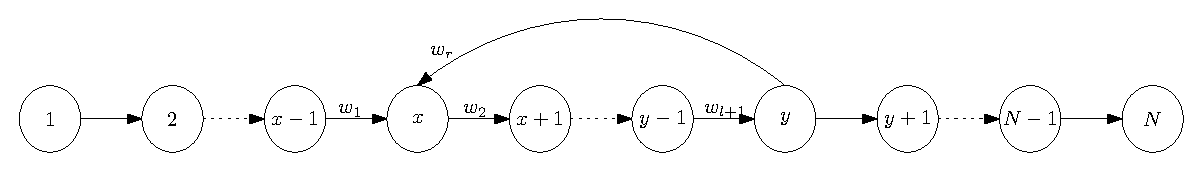
\includegraphics[scale=0.35,keepaspectratio]{Images/EdgeScaling.eps}
		%\caption{Edge Scaled Network}
		\label{EdgeScaledNetwork}
	\end{figure}
	$\Tilde{\mathcal{C}}=\tiny{\begin{bsmallmatrix}
		w_1+w_r  & 0 & \dots & -w_r \\
		-w_2 & w_2 & \dots & 0 \\
		\vdots & \vdots  & \ddots & \vdots \\
		\vdots & \dots & -w_{\ell+1} & w_{\ell+1}
	\end{bsmallmatrix}}$,~~where, $w_i's, i \in \{1,2,\dots,\ell+1\}$ are the forward edge weights and $w_r$ is the forward and reverse edge weight to node $x_1$.\\
	\vspace{-0.2cm}
	\begin{block}{Objective}
		Applying Gershgorin's Disc theorem to columns of $\tilde{\mathcal{C}}$ 
		\vspace*{-0.3cm}
		$$w_1+w_r>w_2>w_3>\dots>w_r$$		
		%\vspace*{-0.15cm}
		- Ensure it is separated from origin \\
		- Maximize the distance of closest disc\\
		\textcolor{blue}{Solution: }Create an Arithmetic Progression between the elements of inequality above.
	\end{block}
	\vspace*{-0.1cm}
	Consensus achieved if:
	$w_1=\frac{\ell+1}{\gamma^2}+\epsilon; w_k=w_1+(k-1)[w_1/(\ell+1)]$, for any $\epsilon>0$ and $k\in\{2,\ldots,\ell+1\}$. \hyperlink{ESSim}{\beamerbutton{Simulations}}~~\hyperlink{gersback}{\beamerbutton{Back2Approach2}}	
	%\end{minipage}
\end{subframe}



\begin{subframe}\label{CombScal}
	\begin{block}{Combined Scaling}
		$$\Tilde{P}=P\Tilde{\mathcal{C}}=\tiny{\begin{bsmallmatrix}
				p_1(w_1+w_f)  &  0 & \dots & -p_1w_1 \\
				-p_2w_2 & p_2w_2 & \dots & 0 \\
				\vdots & \vdots  & \ddots & \vdots \\
				\vdots & \vdots  & -p_{\ell+1}w_{\ell+1} & p_{\ell+1}w_{\ell+1}
		\end{bsmallmatrix}}$$
		where $P$ is the matrix coming from Node Scaling and $\mathcal{C}$ is the matrix coming from Edge Scaling.\\
	\end{block}
	Applying Gershgorin's theorem, we get:\\
	$$p_1(w_1+w_r)>p_2w_2>p_3w_3>\dots>p_1w_r$$
	\textcolor{blue}{Solution: }Create an AP between $p_1(w_1+w_r)$ and $p_1w_r$\\
	\pause
	Why Combine?\\
	\pause
	\textcolor{blue}{Reason:\\ }
	- Greater freedom in parametric choice \\
	- Trade-off between the node and edge scaling parameters.\\
	~~\hyperlink{gersback}{\beamerbutton{Back2Approach2}}
\end{subframe}
	%\pause
	%\hrule
	
	
\begin{subframe}{Directed cycle with root node}
	\textcolor{red}{Will ESS or NSS work for directed cycles with leader ??} \pause \textcolor{blue}{No!! but why ??}\\
	\begin{block}{}
		\begin{itemize}
			\item The edge scaling fails since the edge connecting node $x_1=1$ to $x_1-1$ does not exist (node $0$ is non-existent)
			\item The node scaling method fails because $\Tilde{\mathcal{C}}$ becomes a circulant matrix with a zero eigenvalue, and union of Gershgorin's discs always contains any open neighborhood of the origin.
		\end{itemize}
	\end{block}
	\pause
	\centering
	\textcolor{red}{Solution??} 
	Root Locus Based Methodology ~~\hyperlink{RLSimbase}{\beamerbutton{RLS Method}}
\end{subframe}


\begin{subframe}{Root Locus Method}\label{RLSimbase}
	\vspace*{-0.2cm}
	Choose Node Scaling based approach to scale all but one with scaling factor $\alpha$ and this one node scaling parameter(say for agent $2$) be $\beta$. Then,
	$\Tilde{\mathcal{C}}=\tiny{\begin{bsmallmatrix}
		\alpha  & 0 & \dots & -\alpha \\
		-\beta & \beta & 0 & 0 \\
		\vdots & \vdots & \ddots & \vdots \\
		\vdots & \dots & -\alpha & \alpha
	\end{bsmallmatrix}}$\\
	the $\gamma$ bound as mentioned earlier is driven by the roots of characteristic equation of $\mathcal{C}$ which is given by:\\
	--Characteristic Equation $\chi(s)=1-G(s)=0$, with $G(s)=\frac{\beta\{(s-\alpha)^\ell-(-\alpha)^\ell\}}{s(s-\alpha)^\ell}$.\\
	--Cast as complementary root locus on gain $\beta$.\\
	--Zeros at $\alpha(1-e^{(\iota \frac{\pi}{\ell}(2k))})$ with $k\in\{0,\ldots,\ell-1\}$, where $\iota=\sqrt{-1}$.\\
	\textbf{Note: } The pole at origin is canceled by zero at origin of the G(s).
	\vspace*{-0.2cm}
	\begin{block}{Algorithm}\label{Algo}
		\begin{enumerate}
			\item Choose $\alpha>\frac{1}{\gamma^2}$ and draw the complementary root locus of G(s).
			\item Take it's mirror image by drawing the root locus of G(-s) and shift it by a distance $d=\frac{1}{\gamma^2}$.
			\item Find the gain value at which it remains inside the left half plane.%(\textcolor{red}{It is not equivalent to gain value when it moves to right half})
			\item choose any $\beta$ from that range to guarantee the consensus.
		\end{enumerate}
	\end{block}  
\end{subframe}

%%%%%%%%%%%%%%%%%%%%%%%%%%%%%%%%%%%%%%%%%%%%%%%%%%%%%%%%%%%%%%%%%%%%%%%%%%%%%%%%%%%%%%%
\begin{subframe}{Remarks on Root Locus Approach}
	\begin{enumerate}
		\item Contrary to the node scaling and the edge scaling methods, where increasing the scaling parameters assists in consensus, here the gain $\beta$ needs to be bounded above, while $\alpha$ is to be chosen large.
		\item Note, $\beta=0$ is not a feasible choice, since it implies breaking the cycle that was formed by the reverse edge and is tantamount to dropping an edge altogether, in response to an additional reverse edge.
		\item In most of the literature dealing with consensus in case of perturbed edge weights, such perturbations have mostly been viewed as undesirable, both for undirected and directed graphs. However, we show that a judiciously chosen \emph{perturbation} may also lead to local remedies for a consensus-seeking network of double integrators.
	\end{enumerate} 
	\hyperlink{RLSim}{\beamerbutton{Simulations}}~~\hyperlink{gersback}{\beamerbutton{Back2Approach2}}   
\end{subframe}
%%%%%%%%%%%%%%%%%%%%%%%%%%%%%%%%%%%%%%%%%%%%%%%%%%%%%%%%%%%%%%%%%%%%%%%%%%%%%%%%%%
\begin{comment}
\begin{frame}{Conclusion}
	\begin{block}{Remark on Root locus}
		\begin{itemize}
			\item Need Small $\beta$ unlike node and edge based scaling.
			\item Ideal choice $\beta=0$, \textcolor{red}{Not an appropriate choice}
			\item Edge Perturbation- \textcolor{red}{Bane or Boon?}
		\end{itemize}
	\end{block}
	\begin{block}{Solution to Challenges in Approach 1:}
		\begin{enumerate}
			\item Fails with leader in the directed cycle. \checkmark
			\item Ease computation but not helpful reducing or eliminating the bound. \checkmark
			\item Not a local remedy. \checkmark
			%\paused
		\end{enumerate}
	\end{block}	
	%\pause
	
\end{frame}

\end{comment}



\begin{subframe}{Node Scaling Simulations}\label{NSSim}
	-- Effective length of cycle= $\ell+1=6$ and $\gamma^2=0.16$, Hence, $p_1 \geq \frac{6}{0.16}=37.5$\\
	-- We chose, $p_1=39$, with $diff=39/6=6.5$ and hence, $$P= \text{diag}(39,71.5,65,58.5,52,45.5)$$
	\begin{figure}[ht]
		\centering
		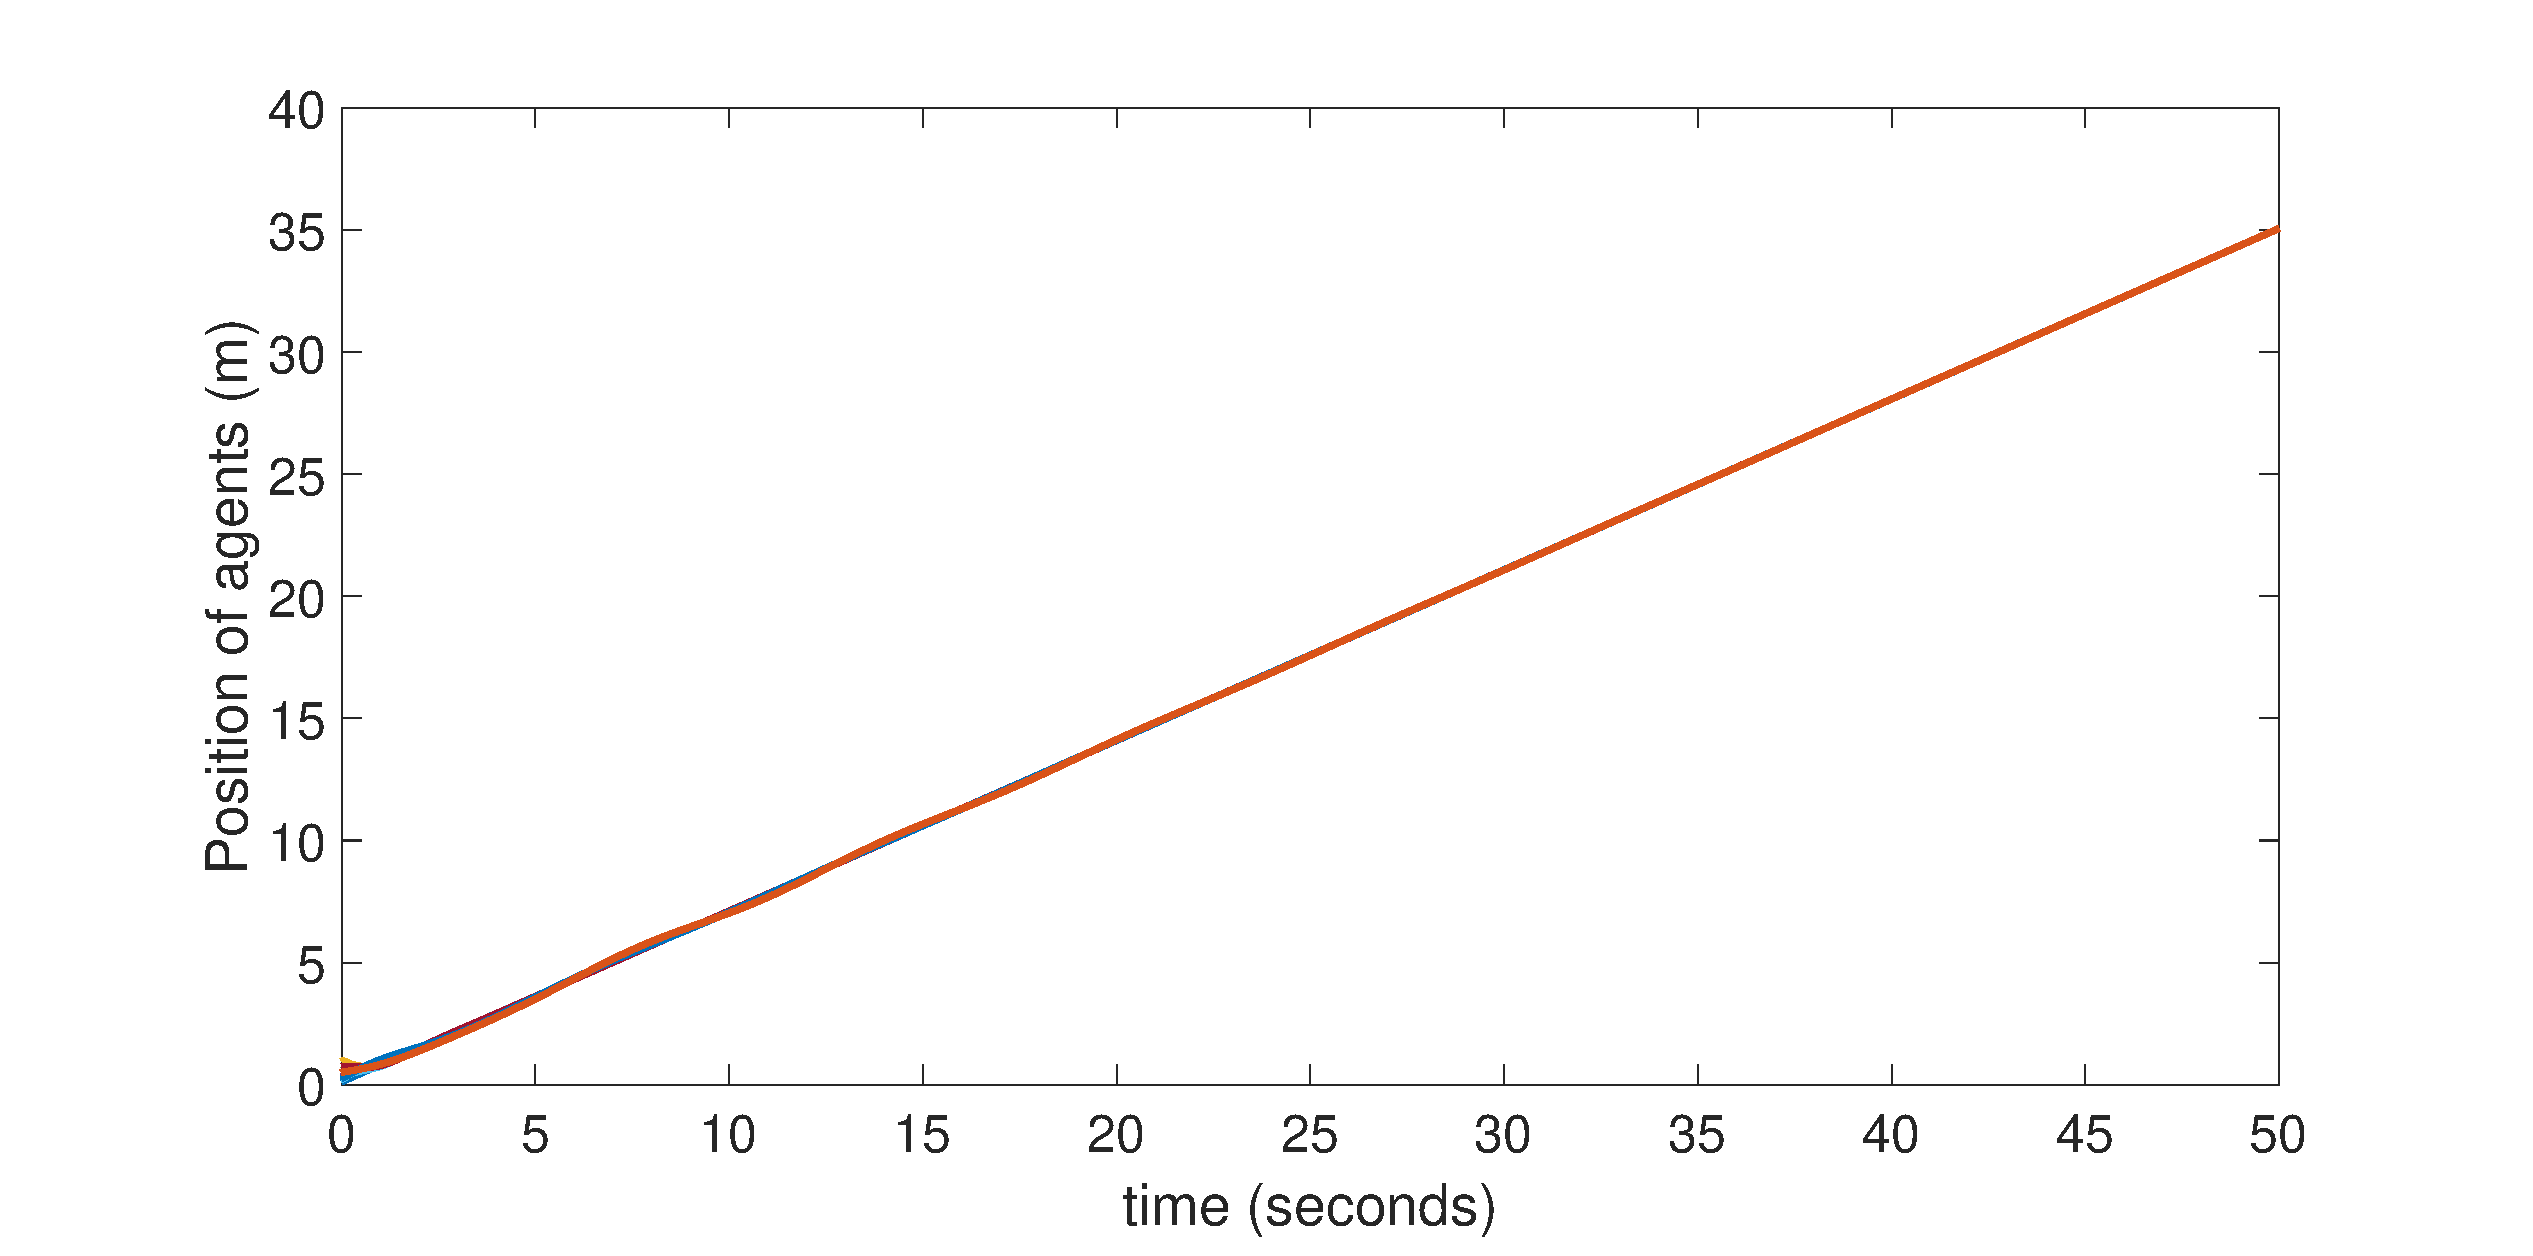
\includegraphics[scale=0.2,keepaspectratio]{Images/9-7-2_NodeScaledlLaplacianGamma0.4PositionConsensus1.eps}
		\caption{Position consensus with node scaled Laplacian for $\gamma = 0.4$}
		\label{NodeScaledLaplacianPositionConsensus0.4}
	\end{figure}
	\vspace{-1.2cm}
	\hyperlink{NSSimbase}{\beamerbutton{Back}}
\end{subframe}


%%%%%%%%%%%%%%%%%%%%%%%%%%%%%%%%%%%%%%%%%%%%%%%%%%%%%%%%%%%%%%%%%%%%%%%%%%%%%%%%%%%%%%%
\begin{subframe}{Edge Scaling Simulations}\label{ESSim}
	--Similar to the node scaling method, here  $w_1 \geq 37.5$ \\
	--We chose, $w_1=39$ and assume $w_r=1$, thus giving $diff=39/6=6.5$ and hence, edge weights $$W= \text{diag}(39,32.5,26,19.5,13,6.5)$$
	\begin{figure}[ht]
		\centering
		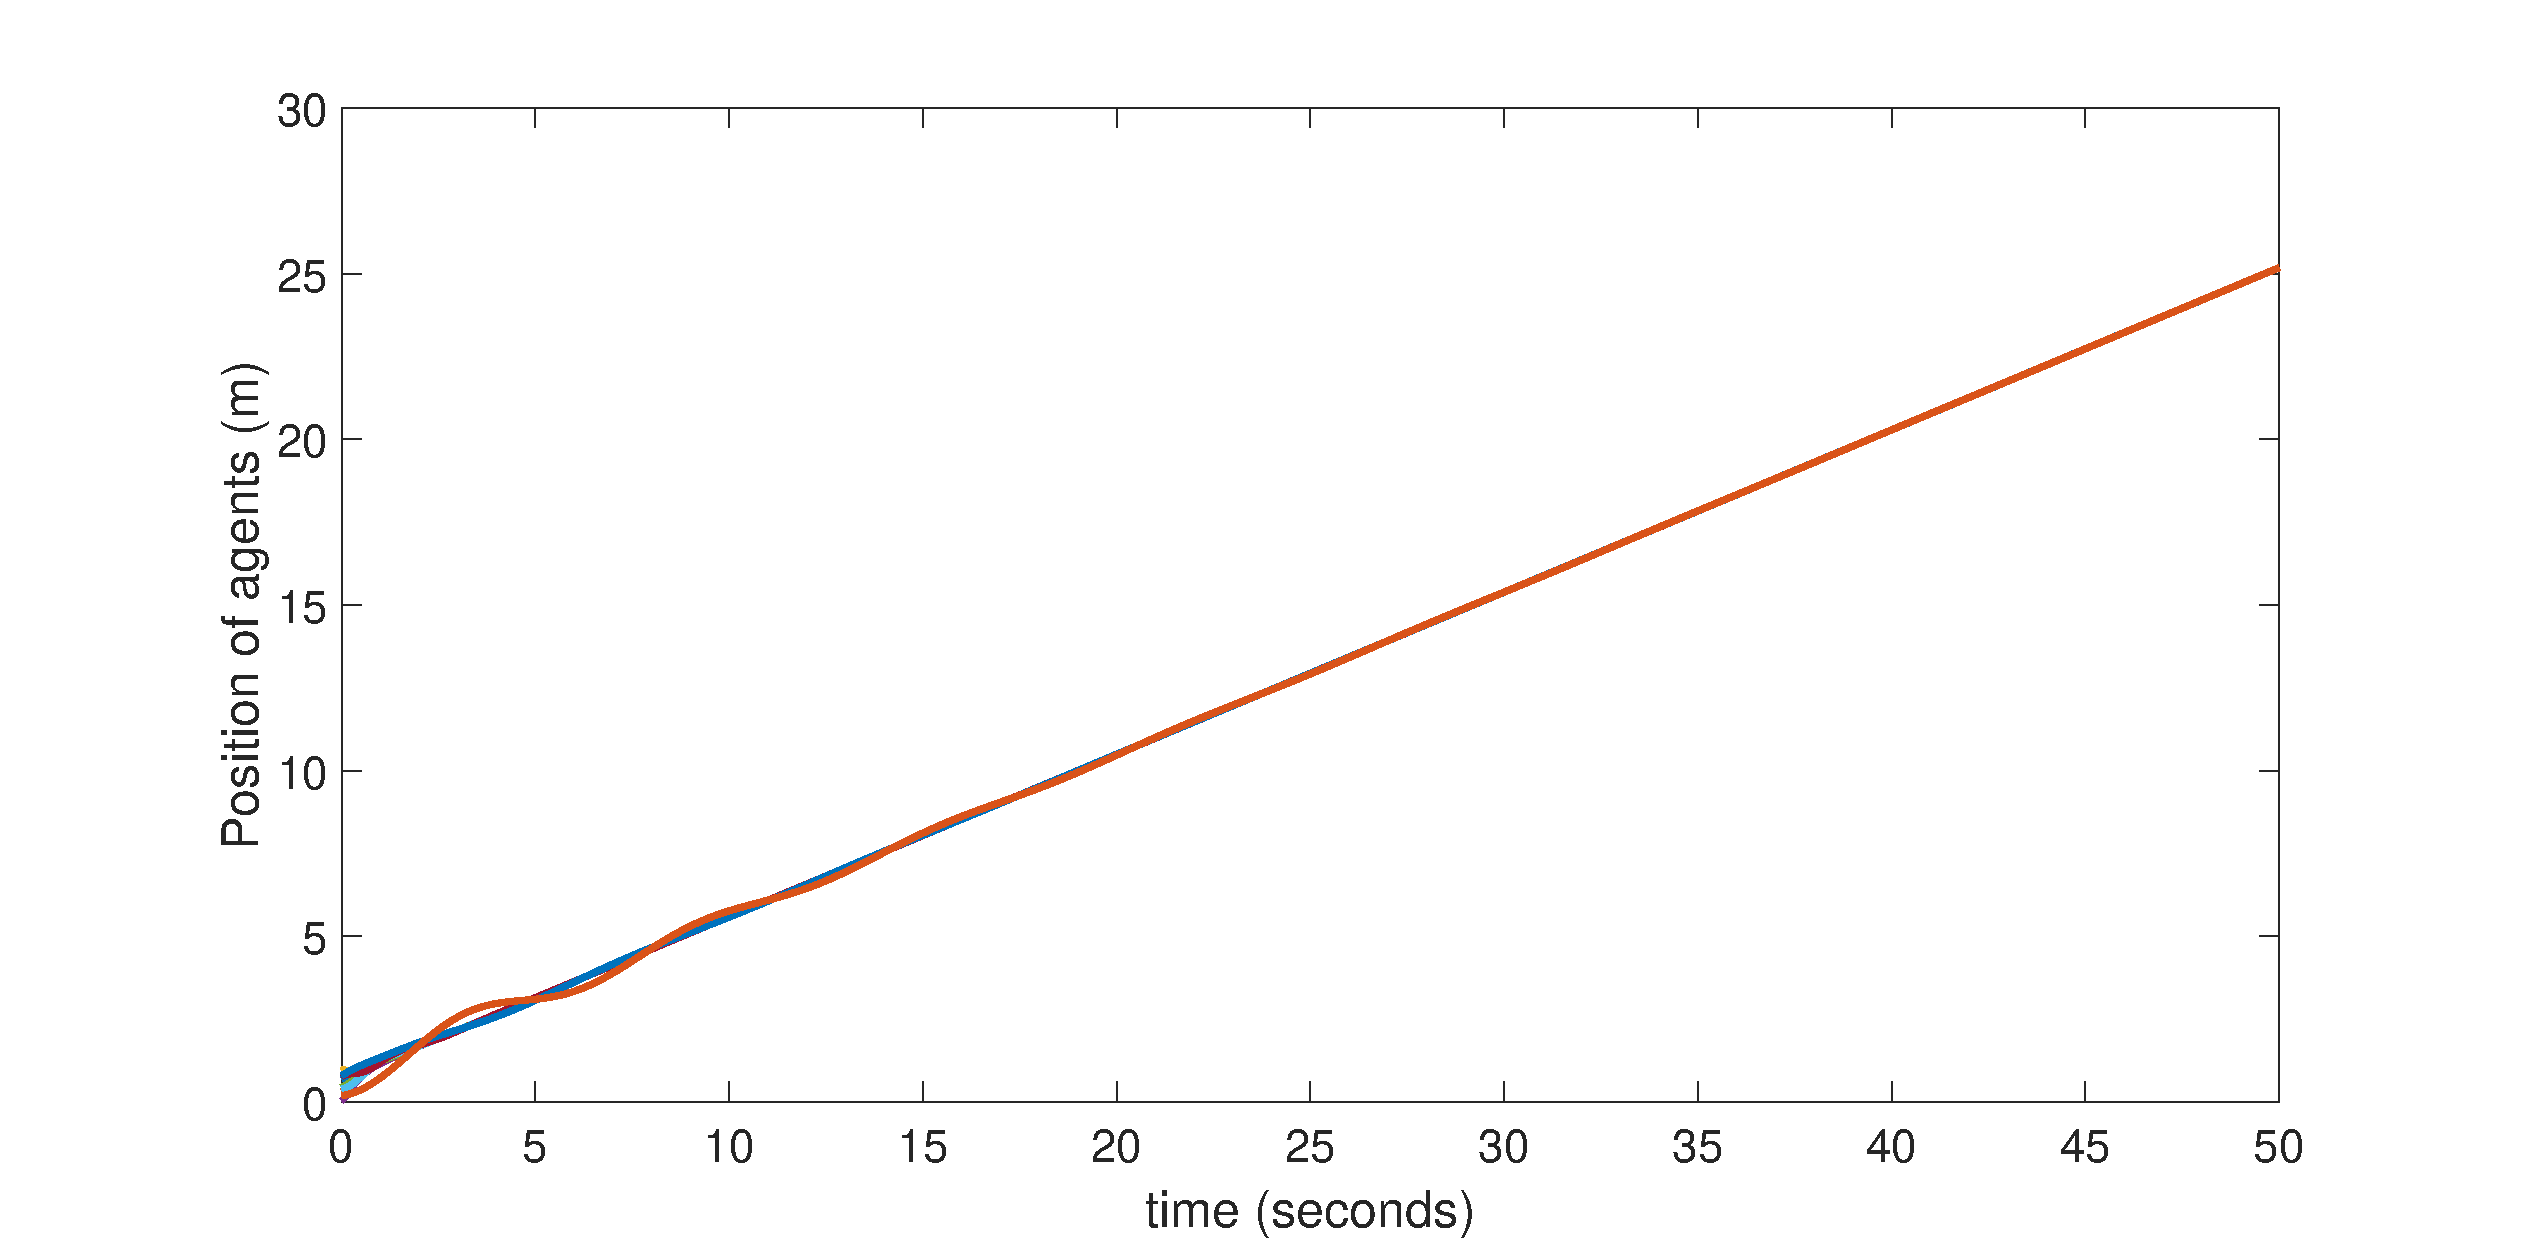
\includegraphics[width=0.5\textwidth,keepaspectratio]{Images/9-7-2_EdgeWeightedlLaplacianGamma0.4PositionConsensus1.eps}
		\caption{Position consensus of edge weight scaled Laplacian with $\gamma = 0.4$}
		\label{EdgeWeightedLaplacianPositionConsensus0.4}
	\end{figure}
	\vspace{-0.3cm}
	\hyperlink{ESSimbase}{\beamerbutton{Back}}
	%\textbf{Note:} Simulation for Combined Method is omitted as it is trivial to achieve consensus but only provides with more flexibility in choosing the design parameters. 
\end{subframe}
%%%%%%%%%%%%%%%%%%%%%%%%%%%%%%%%%%%%%%%%%%%%%%%%%%%%%%%%%%%%%%%%%%%%%%%%%%%%%%%%%%%%%%%


\begin{subframe}{Root Locus Based Simulations}\label{RLSim}	
	We chose $\alpha=10$ and $\tau=9$, and thus from the root locus, we get, $\beta \leq 0.00009$, Thus, we chose $\beta=0.00008$
	\vspace{-0.3cm}	
	\begin{columns}
		\begin{column}{0.5\textwidth}
			\begin{figure}[ht]
				\centering
				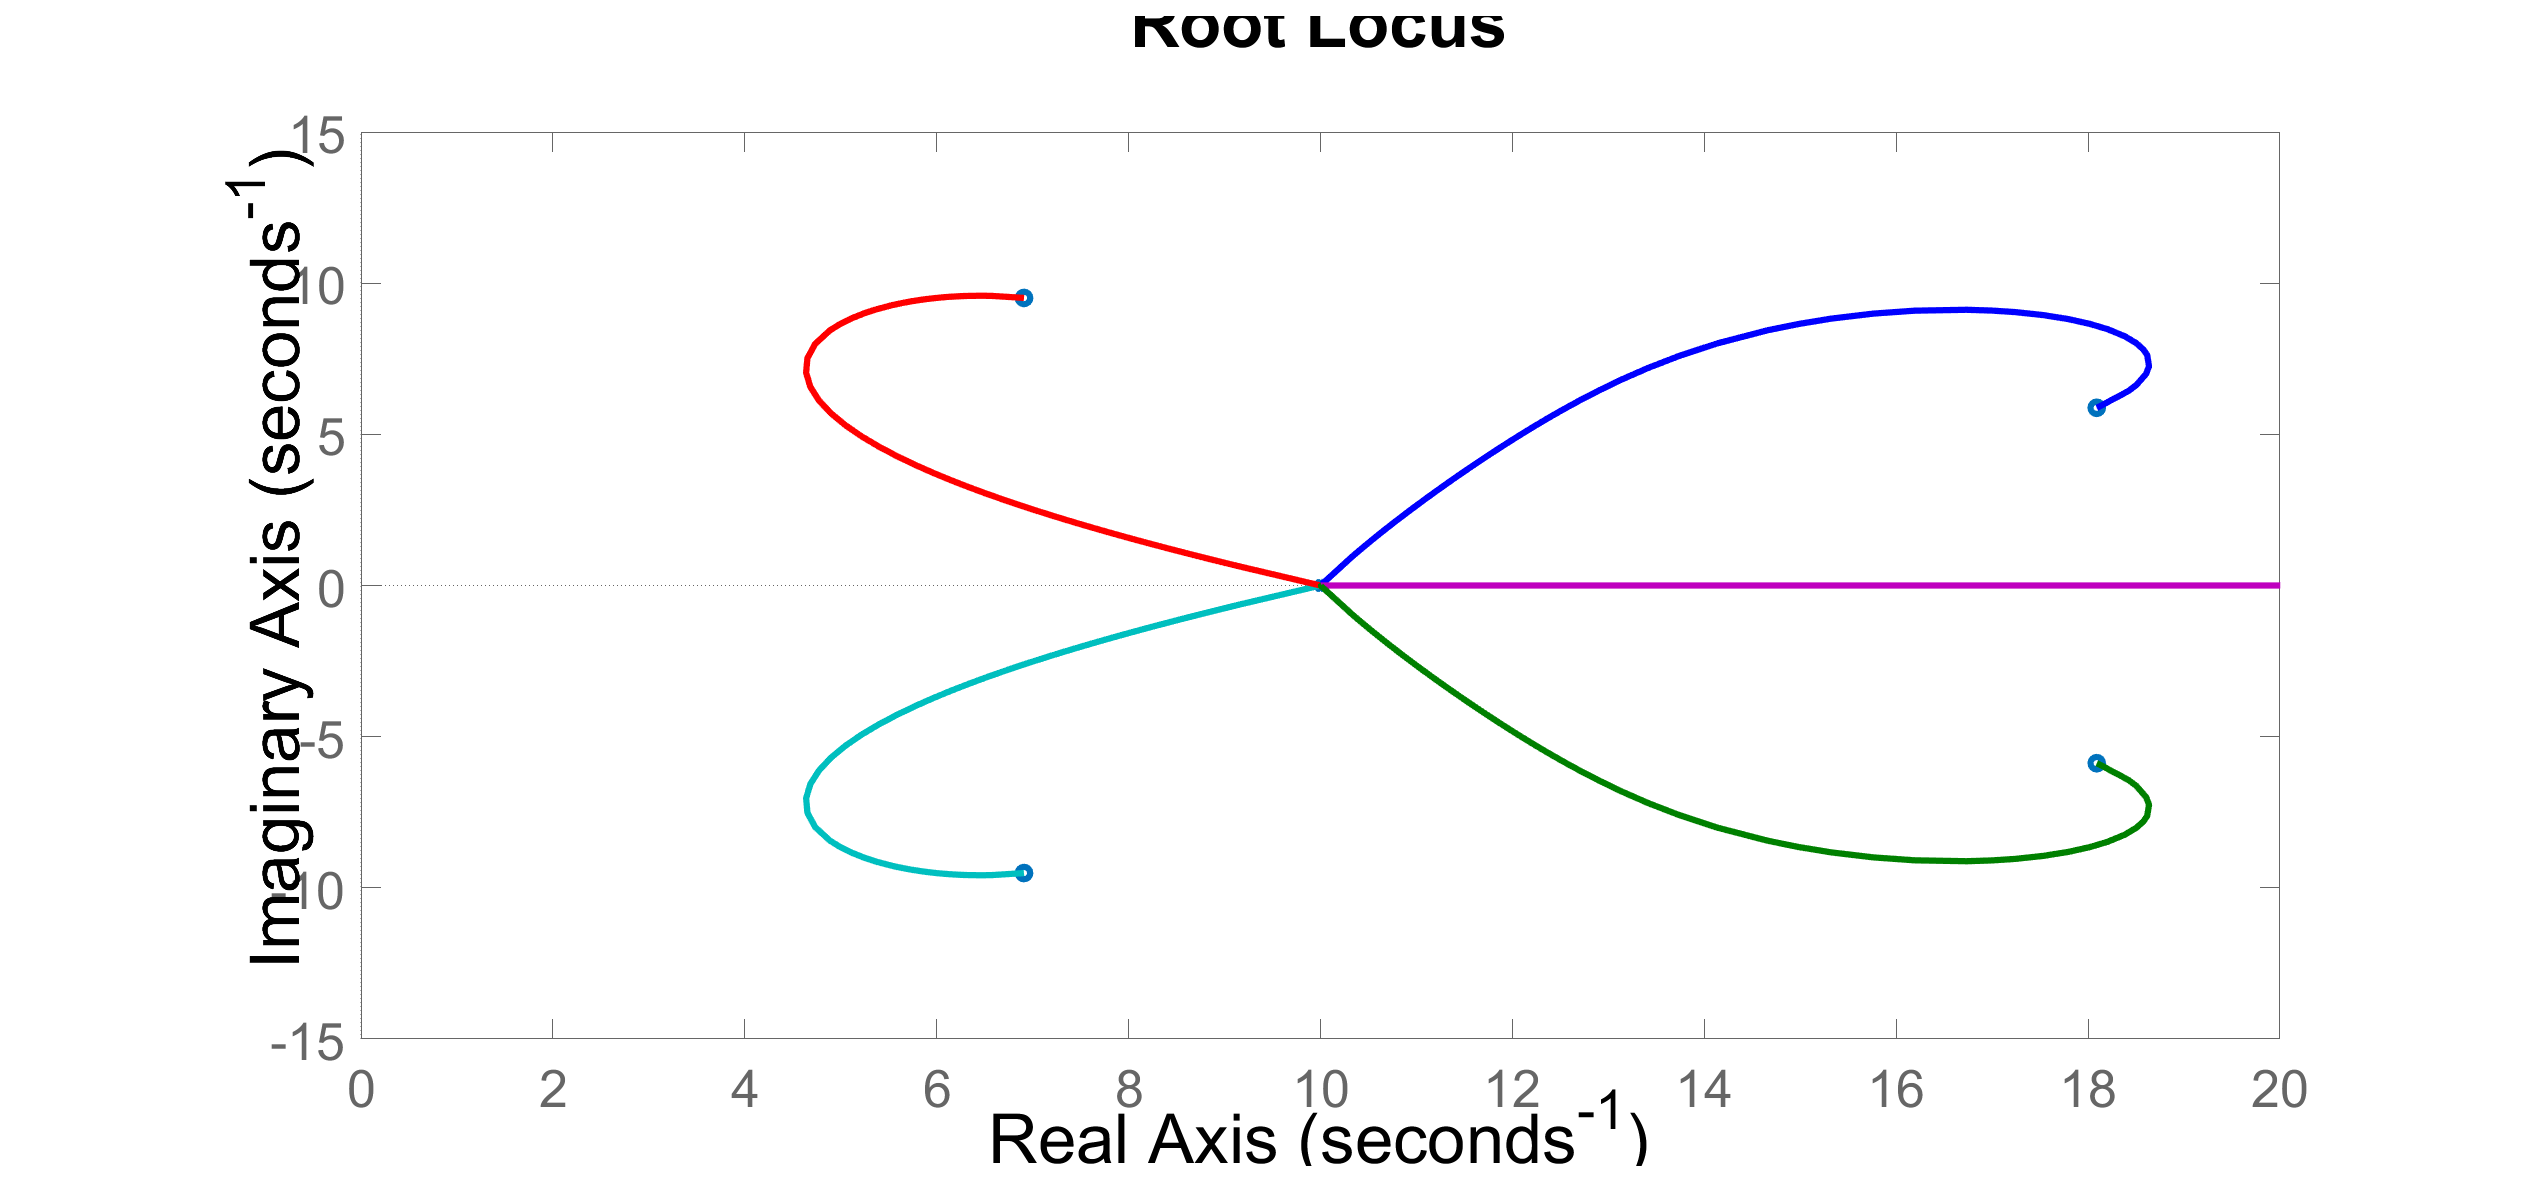
\includegraphics[trim={0 0 0 .6cm},clip,scale=0.18,keepaspectratio]{Images/9-6-1_RootLocus1.eps}
				\caption{Complementary root locus of $G(s)$ when the cycle involves leader}
				\label{ComplimentaryRootLocus}
			\end{figure}
		\end{column}
		\begin{column}{0.5\textwidth}
			\begin{figure}[ht]
				\centering
				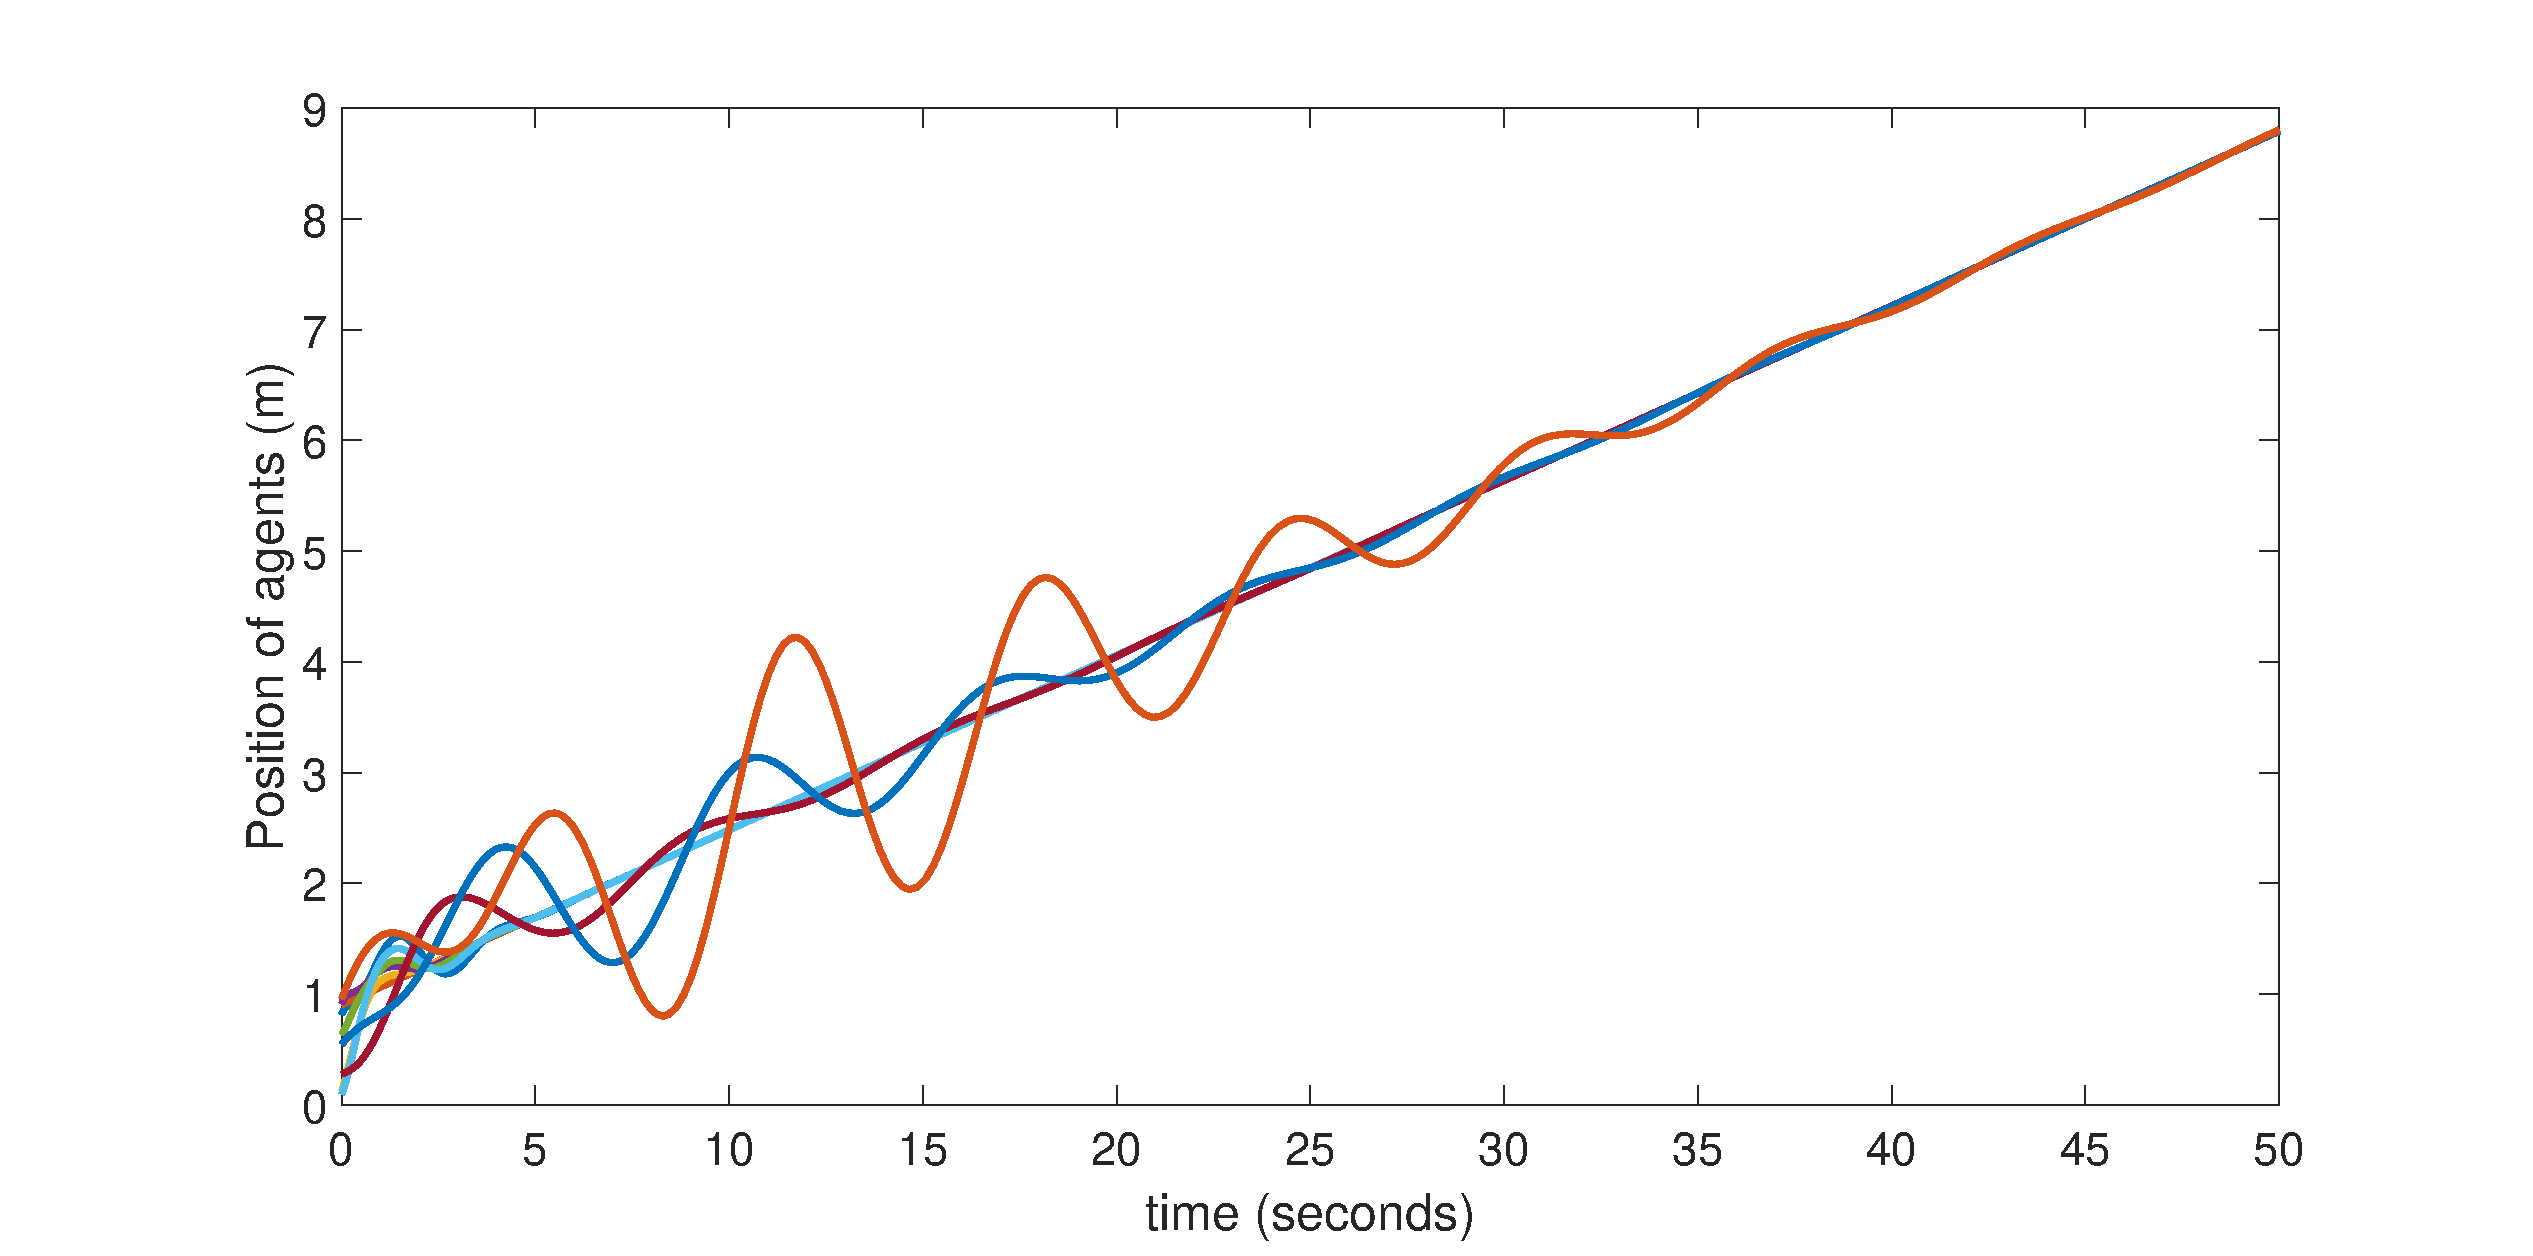
\includegraphics[scale=0.18,keepaspectratio]{Images/9-6-1_RootLocusLaplacianGamma0.4PositionConsensus1.eps}
				\caption{Position consensus with root locus based Laplacian design for $\gamma = 0.4$}
				\label{RootLocusBasedLaplacianPositionConsensus0.4}
			\end{figure}
		\end{column}
	\end{columns}
	%	Parameters chosen based on root locus tuning\\
	%	\begin{minipage}{0.45\linewidth}
		
		%\vspace{-0.3cm}    
		%	\end{minipage}
	%	\hspace{1em}
	%	\begin{minipage}{0.45\linewidth}
		%\vspace{-0.4cm}   
		
		%	\end{minipage}
	%\vspace{-1cm}
	\hyperlink{RLSimbase}{\beamerbutton{Back}}
\end{subframe}
%%%%%%%%%%%%%%%%%%%%%%%%%%%%%%%%%%%%%%%%%%%%%%%%%%%%%%%%%%%%%%%%%%%%%%%%%%%%%%%%%%%%%%%


\begin{subframe}{Gershgorin's Disc Theorem}\label{gers}
	%\begin{minipage}[]{0.4\textwidth}
	\begin{columns}
		\begin{column}{0.5\textwidth}
			Let there be a square matrix $A \in \mathbb{R}^{n \times n}$ and $$R_j(A)=\sum_{i=1,j \neq i}^{i=n}|a_{ij}| \text{ , } \forall \text{ }j \in \{1,2,\dots,n\}$$ $R_j(A)$ is the absolute sum of all the elements except the $j^{\rm th}$ element of column $j$ of matrix $A$. Consider a disc, say $\mathfrak{D}_j$, known as Gershgorin's disc for column $j$, given by $$\mathfrak{D}_j=\{r \in \mathbb{C}:|r-a_{jj}| \leq R_j(A)\}.$$
			Then, the eigenvalues of $A$ lies inside union of all the disks such that $D(A):=\bigcup_{j=1}^{n}\mathfrak{D}_j$.\\
		\end{column}
		\begin{column}{0.5\textwidth}
			\centering	
			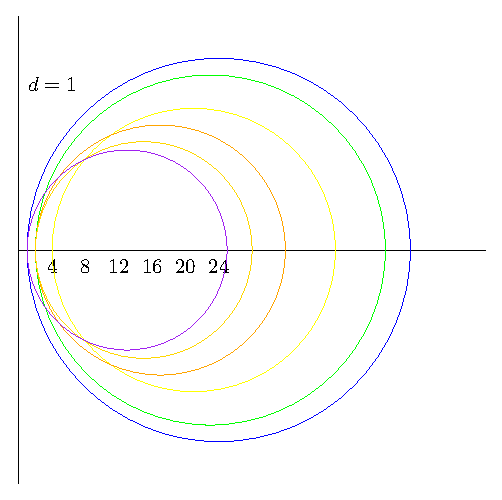
\includegraphics[scale=0.6,keepaspectratio]{Images/GershgorinDiscNotinAP.eps}\\
		\end{column}
	\end{columns}
	%	Let there be a square matrix $A \in \mathbb{R}^{n \times n}$ and $$R_j(A)=\sum_{i=1,j \neq i}^{i=n}|a_{ij}| \text{ , } \forall \text{ }j \in \{1,2,\dots,n\}$$ $R_j(A)$ is the absolute sum of all the elements except the $j^{\rm th}$ element of column $j$ of matrix $A$. Consider a disc, say $\mathfrak{D}_j$, known as Gershgorin's disc for column $j$, given by $$\mathfrak{D}_j=\{r \in \mathbb{C}:|r-a_{jj}| \leq R_j(A)\}.$$
	%	Then, the eigenvalues of $A$ lies inside union of all the disks such that $D(A):=\bigcup_{j=1}^{n}\mathfrak{D}_j$.\\
	%\end{minipage}
	%\begin{minipage}[]{0.5\textwidth}
	%	\centering	
	%	\includegraphics[scale=0.6,keepaspectratio]{GershgorinDiscNotinAP.eps}\\
	%\end{minipage}
	\textbf{Note: }Also true if the \textcolor{blue}{columns and rows are interchanged} since $A$ and $A^T$ have same eigenvalues.	\\
	\hyperlink{gersback}{\beamerbutton{Back}}
\end{subframe}